\section{Project Management}
A project is a temporary organization that has a specific and unique goal and usually a budget (costs, materials, resources).

Project Management is used to manage (plan, monitor, control) the scope, time and cost in order to make the project successful.

\section{Project management processes}
\begin{enumerate}
    \item Initiating
    \item Planning
    \item Executing
    \item Monitoring and controlling
    \item Closing
\end{enumerate}
\subsection{1. Initiating}
\begin{itemize}
    \item Define the project
    \item Define initial scope
    \item Estimate cost and resources
    \item Define the stakeholders
\end{itemize}

\subsection{2. Planning}
\begin{itemize}
    \item Scope management plan: defining, validating and controlling scope
    \item Schedule management plan: how schedule is developed, managed, executed and controlled
    \item Cost management plan
    \item Quality management plan: quality standards, quality assurance and control
    \item Change management plan
    \item Communication management plan
    \item Risk management plan: identify risks and plan responses
\end{itemize}

\subsubsection{Risk Management}
\textbf{Risk} is an uncertain event that if occurs can impact the achievement of objectives.
\begin{itemize}
    \item Risk cause: source (or driver) of the risk
    \item Risk event: uncertain event that might follow the cause
    \item Risk effect: how the objectives might be affected by the risk event
\end{itemize}
Steps for risk management:
\begin{enumerate}
    \item Define roles and responsibilities
    \item Identify possible risks
    \item Give probability (high, low, medium) to each risk
    \item Develop a risk response plan
    \item Define a budget for unknown risks
\end{enumerate}
Type of risks:
\begin{itemize}
    \item Project risks (threaten project plan)
    \item Technical risks (threaten quality and timeliness of product)
    \item Business risks (e.g. market risk, strategic risk, sales risk, management risk, budget risk)
\end{itemize}

\subsubsection{Schedule planning}
Tasks are activities which must be completed to achive the project goal.
Milestones are points in the schedule where progress can be assessed.
Deliverables are work products delivered to the customer (e.g documents).

\begin{enumerate}
    \item Break down project in tasks
    \item Define dependencies between tasks
    \item Define lag time between dependencies (even negative)
\end{enumerate}

\begin{center}
    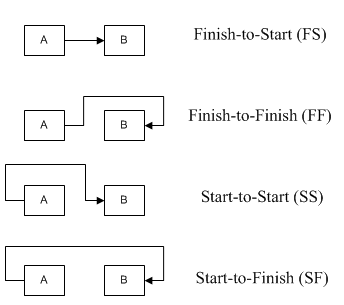
\includegraphics[width=0.6\linewidth]{8-project-management/tasks-dependencies.png}
\end{center}

The critical path is a sequence of tasks that runs from the start to the end of the project.
Changes to task on the critical path changes the project finish date.
A task is critical if it cannot float earlier or later.

Contraints can be:
\begin{itemize}
    \item Flexible (as soon as possible)
    \item Partial flexible (start no earlier than / finish no later than)
    \item Inflexible (must occur on specific time interval)
\end{itemize}

\subsubsection{Cost and Effort estimation}
Two types of techniques: experience-based techniques (based on past projects) and algorithmic cost modelling (formulaic approach).

Estimation changes based on number of COTS and components, programming language used, distribution of the team etc.
Exact size can only be known when project is finished.
\begin{center}
    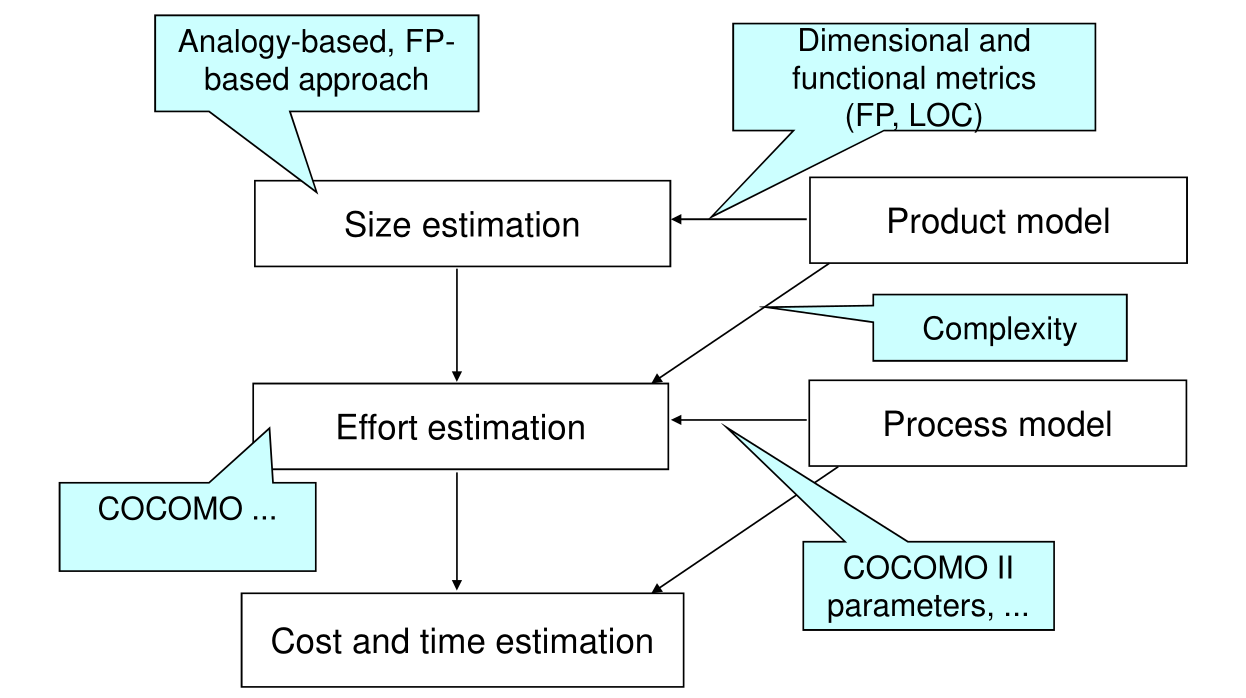
\includegraphics[width=\linewidth]{8-project-management/estimation.png}
\end{center}

\subsubsection{Function Points}
Characterize software dimension basing on functionalities.

Function types:
\begin{itemize}
    \item Internal Logical File (ILF): homogeneous set of data used and managed by the application.
    \item External Logical File (ELF): homogeneous set of data used by the application but maintained by others.
    \item External Input: elementary operation to elaborate date coming from external environment.
    \item External Output: elementary operation that generates data for the external environment (usually includes elaboration of LF).
    \item External Inquiry: elementary operation that involves input and output (without significant elaboration of LF).
\end{itemize}
Every function type is given a weight based on the complexity (simple, medium, complex).
The sum is the Unadjusted Function Points (UFP).
Function points can be used to estimate $LOC = AVC \cdot UFP$, where $AVC$ is language dependent.

\subsubsection{COCOMO II}
Two cases: \emph{Post-Architecture} (extension of existing product) or \emph{Early Design}.
\[ PM = A \cdot Size^E \prod EM_i \]
Where:
\begin{itemize}
    \item $PM$ is Person-Month
    \item $A = 2.94 \frac{PM}{KSLOC}$
    \item $Size$ is the estimated size of the project in $KSLOC$ (Kilo-Source Lines of Code)
    \item $EM$ is \emph{Effort Multiplier} (derived from \emph{Cost Drivers})
    \item $E$ is aggregation of five \emph{Scale Factors}
\end{itemize}

\textbf{Scale Factors}\\
\begin{itemize}
    \item Precedentedness: high if product is similar to previously developed projects.
    \item Dev. Flexibility: high if there are no specific constraints conform to pre-established requirements and external interface specs.
    \item Risk resolution: high if we have a good risk management plan, clear budget and schedule.
    \item Team cohesion: high if stakeholders are able to work in a team.
    \item Process maturity: refers to a well known method for assessing maturity of software organization (CMM, CMMI).
\end{itemize}
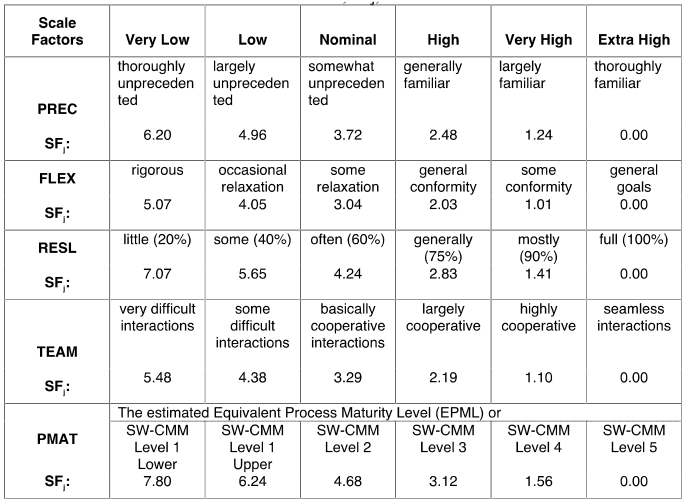
\includegraphics[angle=90,origin=c,width=\linewidth]{8-project-management/scale-factors.png}
\[ E = B + 0.01 \sum_{j=1}^{5} SF_j \qquad B = 0.91 \]

\textbf{Cost Drivers (Post-Architecture)}\\
\begin{itemize}
    \item Product Factors
    \begin{itemize}
        \item Required Software Reliability (RELY)
        \item Data Base Size (DATA)
        \item Product Complexity (CPLX)
        \item Developed for Reusability (RUSE)
        \item Documentation Match to Life-Cycle Needs (DOCU)
    \end{itemize}
    \item Platform Factors
    \begin{itemize}
        \item Execution Time Constraint (TIME)
        \item Main Storage Constraint (STOR)
        \item Platform Volatility (PVOL)
    \end{itemize}
    \item Personnel Factors
    \begin{itemize}
        \item Analyst Capability (ACAP)
        \item Programmer Capability (PCAP)
        \item Personnel Continuity (PCON)
        \item Applications Experience (APEX)
        \item Platform Experience (PLEX)
        \item Language and Tool Experience (LTEX)
    \end{itemize}
    \item Project Factors
    \begin{itemize}
        \item Use of Software Tools (TOOL)
        \item Multisite Development (SITE)
    \end{itemize}
    \item General Factor
    \begin{itemize}
        \item Required Development Schedule (SCED)
    \end{itemize}
\end{itemize}

\textbf{Cost Drivers (Early-design)}\\
\begin{itemize}
    \item PERS (ACAP, PCAP, PCON)
    \item RCPX (RELY, DATA, CPLX, DOCU)
    \item RUSE (RUSE)
    \item PDIF (TIME, STOR, PVOL)
    \item PREX (APEX, PLEX, LTEX)
    \item FCIL (TOOL, SITE)
    \item SCED (SCED)
\end{itemize}

\subsection{3. Executing}
\begin{itemize}
    \item Launch the project : kick off meeting
    \item Acquire and manage project team (internal and \item external resources)
    \item Acquire the required equipment and materials and external services
    \item Execute the plans (communication, change, quality)
    \item Perform the work identified in the WBS
    \item Perform controlling and monitoring activities
\end{itemize}

\subsection{4. Monitoring and Controlling}
Monitoring consists of collecting data about where the project stands, since projects never stick to the initial plans due to changes, problems, etc.
Controlling is where you implement corrections to get your project back on track.
Controlling increases risks factors.
If schedule is important you can use techniques like fast-tracking and crashing
If money is a priority you can reduce costs by reducing resources or overhead costs.
If the schedule, money and resources are not negotiable reduce scope eliminating the tasks associated with it.

\subsubsection{Earned Value Analysis}
\begin{itemize}
    \item Budget at completion (BAC): total budget for the project
    \item Planned value (PV): budgeted cost of work planned
    \item Earned value (EV): budgeted cost of work performed
    \item Actual cost (AC): actual cost for the completed work
\end{itemize}

Behind schedule if $EV < PV$.
Over budget if $EV < AC$.

\textbf{Schedule POV}\\
Schedule Variance: $SV = EV - PV$\\
Schedule Performance Index = $SPI = EV/PV$

\textbf{Cost POV}\\
Cost Variance: $CV = EV - AC$\\
Cost Performance Index = $CPI = EV/AC$

\textbf{Estimate at completion}\\
Spending at the same rate: $EAC = BAC/CPI$\\
Continue to spend at original rate: $EAC = AC + (BAC - EV)$\\
Both CPI and SPI influence remaining work: $EAC = AC + (BAC - EV) / (CPI \cdot SPI)$

\subsubsection{Fast Tracking}
Push tasks to occur faster than they would, by using negative lag time.

\subsubsection{Crashing}
Shorten the tasks on the critical path, usually increases costs.

\subsection{5. Closing}
\begin{itemize}
    \item Ensure project acceptance
    \item Track project performance
    \item Lessons learned
    \item Close contracts
    \item Release resources
\end{itemize}
